\documentclass{school-22.101-notes}
\date{November 23, 2011}

\begin{document}
\maketitle

%%%%%%%%%%%%%%%%%%%%%%% Fermi's Golden Rule %%%%%%%%%%%%%%%%%%%%%%%%%
\subtopic{Fermi's Golden Rule}
Fermi's treatment: beta decay is a transition is caused by weak interaction; it depends on the coupling between the initial state $(i)$ and final state $(f)$. Fermi's Golden Rule is:
\begin{align}
\lambda_{if} &= \frac{2\pi}{\hbar} |M_{if}|^2 \rho_f  & \mbox{Transition Probability} &\sim \mbox{Interaction Matrix} \times \mbox{Density of Final States} \\
M_{if} &= \int_{V} \psi_f^* V \psi_i \dV   &  \psi_f &= \mbox{entire final state after decay} = \psi_D \psi_{\beta} \psi_{\nu} \\
P_{if} &= |M_{if}|^2
\end{align}
We will go over the terms:
\begin{enumerate}
\item $\rho_{f}$ is the density of final states available for find $\frac{\derivative n}{\derivative E_f}$ state. $\rho_f$ describes the number of ways the transition can happen. A transition is more likely to occur if there is a large number of accessible final state. $\rho_f$ depends on energy $T_{\beta}$: 
\begin{align}
\rho_f &= \frac{\derivative n}{\derivative E_f} \\ 
\dn_{e} &\propto p_{e}^2  \dpee_{e} & \dn_{\nu} &\propto p_{\nu}^2 \dpee_{\nu} \\
\dn^2 &= \dn_{e} \dn_{\nu} & \frac{\derivative^2 n}{\derivative E_f^2} &\propto p_{e}^2 p_{\nu}^2 \dpee_{e} \dpee_{\nu}  
\end{align}
%
\item $M_{if}$ is the matrix element for the interaction between the initial and final states. It describes the strength of coupling between initial and final states (higher strength $\to$ stronger coupling $\to$ faster transition).$V$ is an operator describing the interaction which causes the transition. The form of $V$ takes another 20 years to find using experimental results for $N(p)$.
\item To future the discussion on $M_{if}$, consider beta and neutrino as free particles. 
\begin{align}
\psi_{\beta} (r) &= e^{i p_{e} r /\hbar} = 1+ \frac{i p_{e} r }{\hbar} + \frac{1}{2} \left(\frac{i p_{e} r }{\hbar} \right)^2 + \cdots \label{beta-wavefunction}\\
\psi_{\nu} (r) &= e^{i p_{\nu} r /\hbar} = 1+ \frac{i p_{\nu} r }{\hbar} + \frac{1}{2} \left(\frac{i p_{\nu} r }{\hbar} \right)^2 + \cdots 
\end{align}
Given $T_{e} = 1 \MeV$, $T_e = \sqrt{p^2 c^2 + m_e^2 c^4} - m_e c^2 \Rightarrow p_{e} = 1.4 \MeV/c^2 \Rightarrow \frac{p_{e}}{\hbar} = 0.007 \fm^{-1} \Rightarrow \frac{p_e r}{\hbar} \ll 1$. With this approximation,
\eqn{ \psi_e (r) \xrightarrow{\frac{pr}{\hbar} \ll 1} 1, \fsp \psi_{\nu} (r) \xrightarrow{\frac{pr}{\hbar} \ll 1} 1 } 
\textcolor{blue}{This yields the `allowed approximation,' similar to S-wave approximation's assumption of $l=0$. This allowed state is the most likely one. The derived results have no $p_e, p_{\nu}$ dependency.}
\end{enumerate}
Let's put everything together\footnote{Krane Eq.9.25}: 
\begin{align}
\dlambda &\propto |M_{if}|^2 p_{e}^2 p_{\nu}^2 \dpee_{e} \left(\frac{\derivative p_{\nu}}{\derivative E_f} \right)^{1/c} \\
N(p_{e}) \dpee_{e} &= A p_{e}^2 p_{\nu}^2 \dpee_{e} \\
N(p_{e}) &= A p_{e}^2 p_{\nu}^2, \fsp \fsp p_{\nu} =\frac{1}{c} (Q - T_{e}) \\
N(p_{e}) &= A p_{e}^2 (Q - T_{e})^2  = A p_{e}^2 \left[ Q - \sqrt{p_{e}^2 c^2 + m_e^2 c^4} + m_e c^2 \right]^2 \\
N(T_{e}) &\propto T_{e}^2 (Q - T_{e})^2
\end{align}

\uline{Correction}: Fermi's theory gives the right range we want: $N(p) = N(T_e) = 0$ at the minimum and maximum $p$ and $T_e$. The proposed shape is right (Figure~\ref{distribution}), except we need to tweak two things: 
\begin{itemize}
\item $N(T_e = 0) \neq 0$ for $\beta^-$. 
\item $\beta^+$'s spectrum appears to be shifted to the right compared with $\beta^-$. 
\end{itemize} 
\begin{figure}
  \centering
  \subfloat[Predicted]{\label{beta-predict}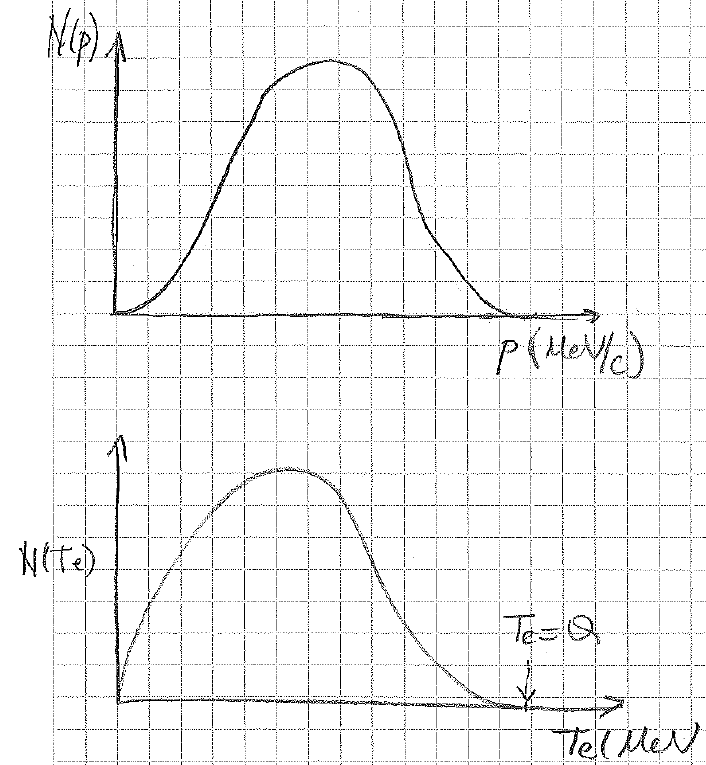
\includegraphics[height=2.7in]{images/rd/beta-predicted-distribution.png}}
  \subfloat[Observed]{\label{beta-predict}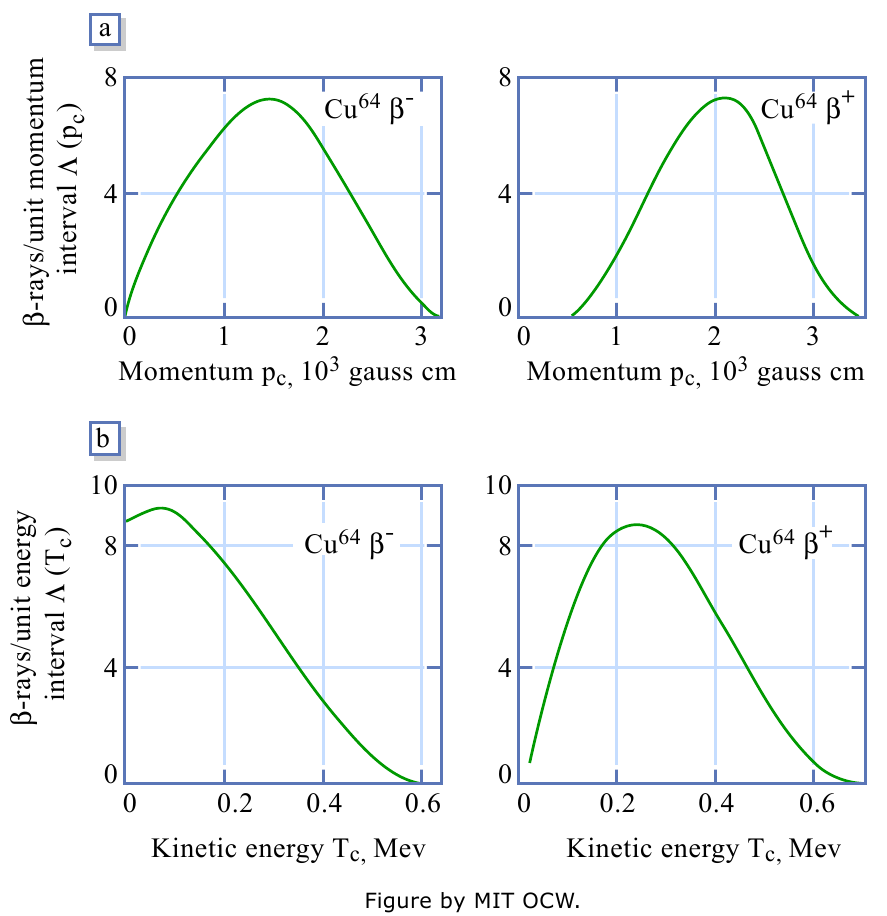
\includegraphics[height=3in]{images/rd/beta-observed-distribution.png}}                  
  \caption{Momentum and Energy Dependency of Neutron Distribution}  \label{distribution}
\end{figure}
Needed correction terms: 
\begin{enumerate}
\item $F(Z^{\prime},p)$ or $F(Z,T_e)$ term (a Fermi function): original model assumes no Coulomb field on $\psi_{\beta}$; we need it to account for Coulomb effect of $\beta^+$ (Coulomb repulsion), $\beta^-$(Coulomb attraction), such that $\beta^+$ would shift the $\beta^-$ spectrum weighted to the right.
\item $S(p_e, p_{\nu})$ term: original model assumes $\frac{pr}{\hbar} \ll 1 \Rightarrow \psi_e \sim \psi_{\nu} \sim 1$, hence no dependence of $M_{if}$ on $p_e, p_{\nu}$. While this assumption is generally valid, it can be wrong sometimes. To correct for it, we need to consider the higher order of $\psi_{\beta}, \psi_{\nu}$ (partial wave). The terms beyond the expansion is commonly called `forbidden decay;' notice they are not absolutely impossible, they are simply with low probability. 
\end{enumerate}
The corrected formula for the distribution of electron momentum (which is proportional to $\lambda(p_e)$) is:
\eqn{N(p_e) = N^o (p_e) \times F(Z^{\prime},p_e) \times S(p_e,p_{\nu}) = C \underbrace{p_e^2 (Q-T_e)^2}_{\textcircled{1}} \underbrace{F(Z^{\prime}, p)}_{\textcircled{2}} \underbrace{|M_{fi}|^2}_{\textcircled{3}} \underbrace{S(p_e, p_{\nu})}_{\textcircled{4}}  }
$\textcircled{1}=$ A statistical factor derived from the density of final states available to the emitted particles; \\
$\textcircled{2}=$ Fermi function to account for the nuclear Coulomb interaction wit the emitted particles;\\
$\textcircled{3}=$ Matrix element for `allowed' ($l_{\beta} = 0$) transition; strength of the interaction between initial and final states; \\
$\textcircled{4}=$ Shape factor to correct $|M_{if}|^2$ for the various `forbidden' transition ($l_{\beta} >0$). 

%%%%%%%%%%%%%%%%% Angular Momentum and Parity %%%%%%%%%%%%%%%%%%
\subtopic{Angular Momentum and Parity Selection Rule}
Nuclear transition must conserve angular momentum and parity, which gives arise to the selection rules below ($I$ is total angular momentum, $L$ is orbital angular momentum, $S$ is spin; subscript $P \sim$ Parent, $D \sim$ Daughter):
\begin{align}
I_P &= I_D + L_{\beta + \nu} + S_{\beta +\nu} \\
\Pi_P &= \Pi_D (-1)^{L_{\beta + \nu}}
\end{align}
\begin{enumerate}
\item The lowest $L$ value corresponds to the most likely state, because $L \down$, $\lambda \up$. Reason: as in Eq.~\ref{beta-wavefunction}, the higher $L$ is, the higher order the expansion is, the less likely the term is, hence we consider the $L=l$ term as l-th forbidden (if $L=0$, we call it allowable). 
\item $\lambda_{\beta} = \lambda (L=0) + \lambda (L=1) + \cdots$, in which $\lambda_{\mathrm{allowed}} \gg \lambda_{\mathrm{forbidden}}, t_{1/2,\mathrm{allowed}} \ll t_{1/2,\mathrm{forbidden}}$. Beta decay's $t_{1/2}$ range from milliseconds to $10^{16}$ years because of the ease in undergoing decay when $l=0$, and the difficulty in doing so when $l>0$. 
\item $S$ can be 0 or 1 (because $S_e = S_{\nu} = \frac{1}{2}$); $S = 0$ is called Fermi decay (F); $S=1$ is called Gamow-Teller decay (G.T.).
\end{enumerate}
Examples:
\begin{itemize} 
\item \ce{^{14}_8 O_6 \to ^{14}_7 N_7^*}. 
    \begin{itemize} 
    \item Spin: $0^+ \to 0^+$, that is, $+ = + (-1)^{L_{\beta + \nu}} \Rightarrow L_{\beta + \nu} = $ even. 
    \item $ 0 = 0 + L_{\beta + \nu}+ S_{\beta + \nu}$. We can have: $(L, S) = (0,0), (1,1)$. From the requirement of the last bullet point, $S=0$ is called the Fermi transition, $L=0$ is the `allowed' one; whereas $L=1$ is the 1st forbidden.  
    \end{itemize}
\item \ce{^{10}_4 Be_6 \to ^{10}_5 B_5}, $3^+ \to 0^+$
    \begin{itemize}
    \item $+ = +^L$, L is even;
    \item $3 = 0 + L + S$. $L = 0$ does not work; $L = 2$ is possible with $S=1$, $L = 2$ is called the 2nd forbidden. 
    \end{itemize}
\item \ce{^{115} In \to ^{115} Sn}, ($\frac{9}{2}^+ \to \frac{1}{2}^+ $)
    \begin{itemize}
    \item $+ = + (-1)^L$, L is even;
    \item $\frac{9}{2} = \frac{1}{2} + L + S$: L cannot be 0 or 2. $L =4,$ S can be either 1 or 0. $L = 4$ is the 4th forbidden, and $S = 1, 0$ are the Fermi and something-else transition. 
    \end{itemize}    
\end{itemize}


%%%%%%%%%%%%%%%%%%%%%%%%%%%%%%% Gamma Decay %%%%%%%%%%%%%%%%%%%%%%%%
\topic{Gamma Decay}
\subtopic{Energetics}
Gamma ray is made of photons of electromagnetic radiation. There is a mass-energy difference from the excited state and the ground state (even though they have the same number of neutrons and protons), and this energy is the available energy before gamma decay, or the energy release after the gamma decay.
\begin{align}
M^* c^2 &= Mc^2 + T_R + E_{\gamma} \\
Q_{\gamma} &=  (M^* - M)c^2  = T_R + E_{\gamma} \\
|P_R| &= |P_{\gamma}| = \hbar k \\
T_R &= \frac{P_R^2}{2M} = \frac{P_{\gamma}^2}{2M} = \frac{\hbar^2 k^2 c^2}{2Mc^2} = \frac{E \gamma^2}{2Mc^2} 
\end{align}
 R stands for recoil, so $T_R, P_R$ are the KE and momentum of the recoiled mass $M$. Since gamma ray is photons, we can use $P_{\gamma} = \hbar k$. 
 
A typical range of gamma energy is: $E_{\gamma} \approx 0.1 \sim 10 \fsp \MeV$. With $2Mc^2$ on the order of $2000 A$ MeV, $T_R$ is very small. Then $Q = E_{\gamma} + T_R \approx E_{\gamma}$.

\subtopic{Gamma Decay Probability}
\begin{align}
\lambda &= \mbox{Probability per unit time for photon emission } = \frac{P}{\hbar \omega} = \frac{\mbox{Power radiated}}{\mbox{photon energy}} \\
P&= f[L,\omega] \cdot |m_{fi} (\sigma L)|^2 = \mbox{power radiated in the EM field} \cdot \mbox{multipole moment} \\
m_{fi} (\sigma L) &= \mbox{multipole transition operation} = \int_V \psi_f^* m(\sigma L) \psi_i \dV, \fsp \fsp \sigma = \mbox{E or M} 
\end{align}

\subtopic{Angular Momentum and Parity Selection Rule}
\begin{align}
I_i &= I_f + I_{\gamma}, S_{\gamma} = 1 \\
\Pi_i &= \Pi_f (-1)^{I_{\gamma}}, I_{\gamma} = L_{\gamma} + S_{\gamma} \\
&\begin{dcases*}
\Pi_{\gamma} = (-1)^{I_{\gamma}} & Electric Multiple \\
\Pi_{\gamma} = (-1)^{I_{\gamma} +1 } & Magnetic Multiple
\end{dcases*} \label{Parity-assignment-gamma}
\end{align}
Example: consider $2^+ \to 0^+$. Then we have : 
\begin{itemize}
\item $2 = 0 + I_{\gamma}, \Rightarrow I_{\gamma} = 2$, given $S=1$, then $L_{\gamma} = 1,2$. 
\item $+ = +(-1)^{2}$ works, hence it has to be electric multiple. 
\end{itemize}
\subtopic{Angular Momentum and Parity Selection Rule, Alternative Approach}
\begin{itemize}
\item Figuring out $L_{\gamma}$ from: $I_i = I_f + L_{\gamma} \Rightarrow L_{\gamma} = |I_i - I_f|, \cdots |I_i + I_f|$. A couple of rules about $L_{\gamma}$: $L_{\gamma} \ge 1$ (this is the reason $0^+ \to 0^+$ is forbidden); decay constant for lower mode is significantly larger than higher modes ($\lambda (M1) \gg \lambda(M2) \gg \cdots; \lambda(E1) \gg \lambda(E2) \cdots$.
\item Figuring out which mode (E or M) based on parity: we either use Eq.\ref{Parity-assignment-gamma}, which is equivalent to:
    \begin{itemize}
    \item Odd parity: E for odd $L_{\gamma}$, M for even $L_{\gamma}$. 
    \item Even parity: E for even $L_{\gamma}$, M for odd $L_{\gamma}$. 
    \end{itemize}
\item Example: $\frac{1}{2}^- \to \frac{1}{2}^+$. L can only be 1 (remember L cannot be 0!). Then from Eq.~\ref{Parity-assignment-gamma}, we want $-1 = (-1)^L$, which is electric. The decay mode is E1. 
\end{itemize}








\end{document}
